% LLNCS macro package for Springer Computer Science procedings;
% Version 2.20 of 2017/10/04
%\documentclass[runningheads]{llncs}
\documentclass[]{llncs} % Using this for now

\usepackage{graphicx} % Still need this for when you add images later
\usepackage{amsmath}  % For math (e.g., the n in N-person)
\usepackage{hyperref} % For clickable links
\hypersetup{
    colorlinks=true,
    linkcolor=blue,
    citecolor=green,
    urlcolor=magenta
}
\usepackage{appendix} % For appendix section

\begin{document}

\title{Navigating the N-Person Prisoner's Dilemma: From the Tragic Valley
  to the Collaborative Hill}
% \titlerunning{N-Person IPD: Tragedy Valley to Reciprocity Hill} % Uncomment if classictype is runningheads

\author{Chris Tcaci and Chris Huyck\inst{1}}
% \authorrunning{C. Tcaci} % Uncomment if classictype is runningheads
\institute{Middlesex University, London NW4 4BT UK\\
\email{M00674787@mdx.ac.uk} \and \email{c.huyck@mdx.ac.uk} \\
\url{https://cwa.mdx.ac.uk/chris/chrisroot.html}
}

\maketitle

%undone are they agents or players

\begin{abstract}
  The N-Person Iterated Prisoner's Dilemma (N-IPD) is an excellent
  environment to explore collaboration. Static agent decision policies
  lead to cooperative results, with high payout when each agent can
  vote against each other agent individually, and the results descend
  into low cooperation when each agent only gets one decision.
  A similar result is shown with agents that learn via reinforcement learning.


\keywords{N-Person Prisoner's Dilemma \and \and Reinforcement Learning \and Emergence of Cooperation \and Multi-Agent Systems.}
% Agent-Based Modelling  \and Tragic Valley \and Collaborative Hill 

\end{abstract}

\section{Introduction}
\label{sec:introduction}

The Prisoner's Dilemma (PD) serves as a foundational paradigm in game
theory, illustrating the conflict between individual rational
self-interest and mutually beneficial collective action
\cite{Axelrod}.  In its simplest form, two individuals, unable to
communicate, must independently choose whether to cooperate or
defect. While mutual cooperation yields a good outcome for both, each
player has an individual incentive to defect, leading to a suboptimal
outcome if both choose to do so. The Iterated Prisoner's Dilemma
(IPD), where the game is played repeatedly, opens the door for
cooperation to emerge through strategies based on reciprocity, as
famously demonstrated by Axelrod's tournaments where Tit-for-Tat
proved remarkably successful \cite{Axelrod}.

However, many real-world social and economic dilemmas—ranging from
managing common resources to international climate agreements—involve
more than two interacting parties. The N-Person Iterated Prisoner's
Dilemma (N-IPD) generalizes the IPD to scenarios with $N$ participants
\cite{Hamburger1973}\cite{Hardin1971}.


This paper will first provide a brief background on the N-IPD and
relevant learning approaches (Section \ref{sec:background}). It then
describes

\section{Background and Related Work}
\label{sec:background} 

This section briefly reviews some key concepts from game theory, focusing on the
N-Person Prisoner's Dilemma (N-IPD), and introduces the Agent-Based Modelling
(ABM) and Multi-Agent Reinforcement Learning (MARL) approaches relevant to this
paper. 

\subsection{The Prisoner's Dilemma}
The canonical version of the Prioner's Dilemma was presented by
Axelrod and Hamilton \cite {Axelrod}.  There are two prisoners
and they are given the option to turn the other in.  So both have
the option to collaborate, and not turn the other in, or defect.
That is each has a choice {\it C} or {\it D}.  Each is given a reward
based on their decision and the decision of the other.  If they both
collaborate they both are given $R$, a reward.  If both defect they
are $P$, a punishment.  If one defects, and the other collaborates,
the defector is given $T$, a temptation, and the collaborator is given
$S$, a sucker's payoff.  

\begin {table} [ht]
\begin{center}
  Prisoner 1 \\
    Prisoner 2
  \begin {tabular}{c | c | c |}
& Collaborate &  Defect \\
\hline
Collaborate& $R_{1,2}$ &  $T_1 S_2$ \\
\hline
Defect& $T_2 S_1$ &  $P_{1,2}$ \\
\hline
\end {tabular}
\caption {The table represents the outcomes for the four scenarios when
  two prisoners vote.  When both collaborate, both get $R$, and when
  both defect, both get $P$.  When one collaborates and one defects,
  the defector gets $T$ and the collaborator gets $S$ payoff.}
\label {tabPayoff}
\end {center}
\end {table}

Axelrod and Hamilton restrict the values so that equations \ref {restrict1}
and \ref {restrict2} are followed.  A standard set of values is $T=5$, $R=3$,
$P=1$ and $S=0$.

\begin{equation}\label{restrict1}
T > R > P > S 
\end{equation}
\begin{equation}\label{restrict2}
R > (S + T) / 2
\end{equation}

The IPD merely plays the tournament over and over.  This gives the agents
a chance to develop their own policy.

The Tit-for-Tat (TFT) strategy proved to be most successful.  The
strategy is to collaborate when the opponent collaborates, then
defect in the round after they defect.  Note that the TFT strategy
is not a Nash equilbrium \cite {Nash}, indicating that it can make
cooperation difficult to maintain \cite {Holt}.

\subsection{The N-Person Prisoner's Dilemma (N-IPD)}

The Iterated Prisoner's Dilemma (IPD) serves as a model for
understanding cooperation. While Axelrod's work highlighted the
success of strategies like TFT in two-player encounters,
extending this to multi-agent scenarios (N-Person IPD or N-IPD)
reveals a more complex strategic landscape. This section details our
agent-based modeling framework, the specific experimental
configurations used to explore this landscape, and the metrics for
evaluating outcomes. Our central aim is to contrast how interaction
structure influences cooperative dynamics, leading to what we term the
"Reciprocity Hill" in pairwise settings and the "Tragedy Valley" in
N-Person group settings.

\subsection{Core Interaction Models}
When there are $N$ agents (and they all have only one vote), 
an individual agent's payoff is determined by its
own choice and the total number of other agents in the group who
chose to cooperate. This structure represents scenarios with diffuse
payoffs, where individual actions contribute to a shared outcome, and
direct one-to-one reciprocity is obscured. The payoff for an agent who
cooperates is calculated as $S + (R - S) \times (n_{oc} / (N - 1))$,
and for a defector as $P + (T - P) \times (n_{oc} / (N - 1))$, where
$n_{oc}$ is the number of other cooperators. $T$, $R$, $P$, and $S$ are
from table \ref {tabPayoff}, and the simulations below use the default values,
$T=5$, $R=3$, $P=1$ and $S=0$.

There are  two distinct interaction models in N-IPD environments.
The first is the pairwise voting model. In this setup, agents can
vote for each of the other $N-1$ players.  This is in esence a series of
independent 2-player IPD games. Each round each of the $N$ players plays
against the $N-1$ other players. An
agent's total score is the sum of payoffs from all its interactions. This
model emphasizes direct, one-to-one accountability,
where the actions of one agent in a pair directly affect the other,
and responses can be specifically targeted.

The second is neighbourhood voting model.  All $N$ agents make a
single choice (cooperate or defect) simultaneously as part of one
collective group. In this case payoff comes directly from the individual
interactions of table \ref {tabPayoff}.

\subsection{Agent Strategies and Adaptations}

There are several static polcies that are used.  They are static in
the sense that they perform by the same rules each time.  These are
the always collaborate strategy, the always defect strategy and the
Tit-for-Tat strategy.  In the N-Person game the Tit-for-Tat (TFT)
strategy makes a probabilistic decision based on the number of
collaborators in the last round.  That is, if the number of
collaborating agents in the prior round is $C$, and there are $N-1$
other agents, the TFT agents randomly select collaborate $C/(N-1)$ of
the time.  An additional variant of the TFT agent, the TFT-E agent,
explores; that is a given percentage of the time, no matter what the
other agents do, the TFT-E agent merely flips a coin to determine whether
it collaborates or defects.

\subsection{Agent-Based Modelling (ABM) for Social Dilemmas}
Agent-Based Modelling (ABM) offers a powerful computational
methodology for studying complex social systems from the bottom up
\cite{Gilbert2007, Macal2010}. By simulating the actions and
interactions of autonomous, heterogeneous agents according to
predefined rules within a specified environment, ABM allows
researchers to observe emergent macroscopic phenomena, such as the
rise or fall of cooperation. It is particularly well-suited for
exploring the N-IPD due to its ability to model local interactions,
diverse agent strategies (including learning), and the non-linear
dynamics that often characterize social dilemmas. Axelrod's pioneering
tournaments using ABM for the 2-player IPD provided early insights
into the conditions favoring cooperative strategies \cite{Axelrod}.

\subsection{Reinforcement Learning in Multi-Agent Systems (MARL)}
Reinforcement Learning (RL) is a class of machine learning where
agents learn to make sequences of decisions by interacting with an
environment and receiving feedback in the form of rewards or
punishments \cite{SuttonBarto2018}.  Standard Q-learning is a
foundational RL algorithm that learns the value of taking a particular
action in a given state. However, when applied to multi-agent
systems, where multiple agents are learning simultaneously, standard
RL algorithms face significant challenges, primarily due to the
non-stationarity of the environment: each agent's policy changes as it
learns, thereby changing the environment from the perspective of other
agents \cite{Busoniu2008}.  This can destabilize learning and prevent
convergence to cooperative equilibria. To address these issues within
the N-IPD context, prior work has explored more advanced multi-agent
reinforcement learning (MARL) techniques like Hysteretic Q-learning
\cite{Matignon2007Hysteretic} and WoLF-PHC \cite{Bowling2002WoLF},
which aim to endow agents with more sophisticated learning
capabilities. Our study focuses on simpler reactive strategies and
their adaptations to highlight structural effects.

Q-learning \cite {Watkins} is a system that learns by building tables
of results from prior experience.  For example, in the case below, three
agents participate, and make decisions.  If one is a Q-learning agent,
it can build a table of, for example, the last two moves.  Each step
move has eight possible outcomes $2^3$, so there are 64 cells to fill.
Additionally, the Q-learning agent typically has an explore option,
so that no matter what the tables say, it will try a random move a
small percentage of the time.  


\section{The Collaborative Hill and the Tragic Valley}
\label{sec:tragicValley}

The simplest extension to the two person IPD is the three person IPD.
Simulations on this task show that the voting mechanism largely determines
whether the agents converge on a cooperative solution (the Collaborative
Hill) or whether they defect (the Tragic Valley).

\begin{figure}
\begin{center}
% GNUPLOT: LaTeX picture with Postscript
\begingroup
  \makeatletter
  \providecommand\color[2][]{%
    \GenericError{(gnuplot) \space\space\space\@spaces}{%
      Package color not loaded in conjunction with
      terminal option `colourtext'%
    }{See the gnuplot documentation for explanation.%
    }{Either use 'blacktext' in gnuplot or load the package
      color.sty in LaTeX.}%
    \renewcommand\color[2][]{}%
  }%
  \providecommand\includegraphics[2][]{%
    \GenericError{(gnuplot) \space\space\space\@spaces}{%
      Package graphicx or graphics not loaded%
    }{See the gnuplot documentation for explanation.%
    }{The gnuplot epslatex terminal needs graphicx.sty or graphics.sty.}%
    \renewcommand\includegraphics[2][]{}%
  }%
  \providecommand\rotatebox[2]{#2}%
  \@ifundefined{ifGPcolor}{%
    \newif\ifGPcolor
    \GPcolortrue
  }{}%
  \@ifundefined{ifGPblacktext}{%
    \newif\ifGPblacktext
    \GPblacktexttrue
  }{}%
  % define a \g@addto@macro without @ in the name:
  \let\gplgaddtomacro\g@addto@macro
  % define empty templates for all commands taking text:
  \gdef\gplbacktext{}%
  \gdef\gplfronttext{}%
  \makeatother
  \ifGPblacktext
    % no textcolor at all
    \def\colorrgb#1{}%
    \def\colorgray#1{}%
  \else
    % gray or color?
    \ifGPcolor
      \def\colorrgb#1{\color[rgb]{#1}}%
      \def\colorgray#1{\color[gray]{#1}}%
      \expandafter\def\csname LTw\endcsname{\color{white}}%
      \expandafter\def\csname LTb\endcsname{\color{black}}%
      \expandafter\def\csname LTa\endcsname{\color{black}}%
      \expandafter\def\csname LT0\endcsname{\color[rgb]{1,0,0}}%
      \expandafter\def\csname LT1\endcsname{\color[rgb]{0,1,0}}%
      \expandafter\def\csname LT2\endcsname{\color[rgb]{0,0,1}}%
      \expandafter\def\csname LT3\endcsname{\color[rgb]{1,0,1}}%
      \expandafter\def\csname LT4\endcsname{\color[rgb]{0,1,1}}%
      \expandafter\def\csname LT5\endcsname{\color[rgb]{1,1,0}}%
      \expandafter\def\csname LT6\endcsname{\color[rgb]{0,0,0}}%
      \expandafter\def\csname LT7\endcsname{\color[rgb]{1,0.3,0}}%
      \expandafter\def\csname LT8\endcsname{\color[rgb]{0.5,0.5,0.5}}%
    \else
      % gray
      \def\colorrgb#1{\color{black}}%
      \def\colorgray#1{\color[gray]{#1}}%
      \expandafter\def\csname LTw\endcsname{\color{white}}%
      \expandafter\def\csname LTb\endcsname{\color{black}}%
      \expandafter\def\csname LTa\endcsname{\color{black}}%
      \expandafter\def\csname LT0\endcsname{\color{black}}%
      \expandafter\def\csname LT1\endcsname{\color{black}}%
      \expandafter\def\csname LT2\endcsname{\color{black}}%
      \expandafter\def\csname LT3\endcsname{\color{black}}%
      \expandafter\def\csname LT4\endcsname{\color{black}}%
      \expandafter\def\csname LT5\endcsname{\color{black}}%
      \expandafter\def\csname LT6\endcsname{\color{black}}%
      \expandafter\def\csname LT7\endcsname{\color{black}}%
      \expandafter\def\csname LT8\endcsname{\color{black}}%
    \fi
  \fi
    \setlength{\unitlength}{0.0500bp}%
    \ifx\gptboxheight\undefined%
      \newlength{\gptboxheight}%
      \newlength{\gptboxwidth}%
      \newsavebox{\gptboxtext}%
    \fi%
    \setlength{\fboxrule}{0.5pt}%
    \setlength{\fboxsep}{1pt}%
    \definecolor{tbcol}{rgb}{1,1,1}%
\begin{picture}(7200.00,5040.00)%
    \gplgaddtomacro\gplbacktext{%
      \csname LTb\endcsname%%
      \put(814,704){\makebox(0,0)[r]{\strut{}$0$}}%
      \put(814,1229){\makebox(0,0)[r]{\strut{}$0.2$}}%
      \put(814,1754){\makebox(0,0)[r]{\strut{}$0.4$}}%
      \put(814,2279){\makebox(0,0)[r]{\strut{}$0.6$}}%
      \put(814,2804){\makebox(0,0)[r]{\strut{}$0.8$}}%
      \put(814,3329){\makebox(0,0)[r]{\strut{}$1$}}%
      \put(814,3854){\makebox(0,0)[r]{\strut{}$1.2$}}%
      \put(814,4379){\makebox(0,0)[r]{\strut{}$1.4$}}%
      \put(946,484){\makebox(0,0){\strut{}$0$}}%
      \put(1532,484){\makebox(0,0){\strut{}$5$}}%
      \put(2117,484){\makebox(0,0){\strut{}$10$}}%
      \put(2703,484){\makebox(0,0){\strut{}$15$}}%
      \put(3289,484){\makebox(0,0){\strut{}$20$}}%
      \put(3875,484){\makebox(0,0){\strut{}$25$}}%
      \put(4460,484){\makebox(0,0){\strut{}$30$}}%
      \put(5046,484){\makebox(0,0){\strut{}$35$}}%
      \put(5632,484){\makebox(0,0){\strut{}$40$}}%
      \put(6217,484){\makebox(0,0){\strut{}$45$}}%
      \put(6803,484){\makebox(0,0){\strut{}$50$}}%
    }%
    \gplgaddtomacro\gplfronttext{%
      \csname LTb\endcsname%%
      \put(5816,4206){\makebox(0,0)[r]{\strut{}3-TFT}}%
      \csname LTb\endcsname%%
      \put(5816,3986){\makebox(0,0)[r]{\strut{}2-TFT+D}}%
      \csname LTb\endcsname%%
      \put(5816,3766){\makebox(0,0)[r]{\strut{}2-TFT-E+D}}%
      \csname LTb\endcsname%%
      \put(5816,3546){\makebox(0,0)[r]{\strut{}2-TFT-E+C}}%
      \csname LTb\endcsname%%
      \put(209,2541){\rotatebox{-270.00}{\makebox(0,0){\strut{}Cooperation}}}%
      \put(3874,154){\makebox(0,0){\strut{}Round}}%
      \put(3874,4709){\makebox(0,0){\strut{}Average Cooperation by Round with Pairwise Voting}}%
    }%
    \gplbacktext
    \put(0,0){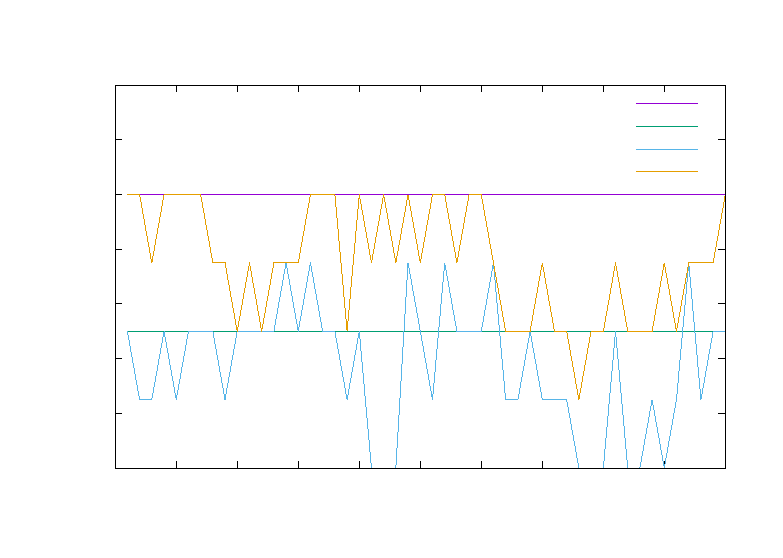
\includegraphics[width={360.00bp},height={252.00bp}]{pairwise}}%
    \gplfronttext
  \end{picture}%
\endgroup
 
\end {center}
\caption{Results from four static 50 round tournaments with
  neighbourhood voting.  3-TFT refers to 3 tit-for-tat agents that
  start cooperating; note that they continue to cooperate.  2-TFT+D
  refers to two tit-for-tat agents with an agent that always defects;
  this leads to system where the TFT agents collaborate with each
  other and defect against the defecting agent.  2-TFT-E+D refers to
  two tit-for-tat agents with 10\% exploration and an always defect
  agent; this leads to a system where the TFT agents have some
  collaboration but mostly defect.  2-TFT-E+C refers to two
  tit-for-tat agents with 10\% exploration and an agent that always
  cooperates; the TFT agents mostly collaborate, but there is some
  defection. }
  \label{figStaticTwoVotes}
\end {figure}


The first set of simulations uses pairwise voting, and tournaments are
run with agents with static policies.  Fifty iteratitions are
performed on four different sets of three agents with static policies:
three Tit-for-Tat (TFT) agents, two TFT with 10\% exploration (TFT-E)
and one always defect, two TFT agents and one always defect agent, and
two TFT-E agents and one always collaborate agent.  The results are
shown in figure \ref {figStaticTwoVotes}.  The vertical axis refers to
how often the two or three TFT or TFT-E agents voted collaborate.  The
Tit-for-Tat agents start off by collaborating, and the three TFT
system continues to collaborate.  The two TFT agents with the always
defect agent always collaborate with each other but (undone, after an
initial collaboration) always defect against the always defect agent.
This leads to a lower average payout, but is still largely
collaborative.  Both of these give horizontal lines in figure \ref
{figStaticTwoVotes}.

The TFT-E agents behave more stochastically, as sometimes they change
their decisions.  The pair with the collaborative agent largely
collaborate, and the pair with the always defect agent largely defect.
Below (figure \ref {figStaticAverage}) it is shown that the ratio is
75\% and 25\%.

The second set of simulations uses neighbourhood voting, with each
agent getting one vote.  The results are shown in figure \ref
{figStaticOneVote}. The same four sets of agents, using static
policies, are used.  The three TFT agents continue to collaborate, as
do the two TFT agents with the always collaborate agent (not shown in
figure \ref {figStaticOneVote}).  However, the TFT agents with the
always defect initially vote to collaborate, but then quickly move to
always defect.  They descend into the Tragic Valley.

The TFT-E systems move up and down, with the pair with the
collaborative agent being more collaborative, and the pair with the
defecting agent being less collaborative.  Below (figure \ref
{figStaticAverage}) it is shown that the ratio is 80\% and 20\% .

\begin{figure}
\begin{center}
% GNUPLOT: LaTeX picture with Postscript
\begingroup
  \makeatletter
  \providecommand\color[2][]{%
    \GenericError{(gnuplot) \space\space\space\@spaces}{%
      Package color not loaded in conjunction with
      terminal option `colourtext'%
    }{See the gnuplot documentation for explanation.%
    }{Either use 'blacktext' in gnuplot or load the package
      color.sty in LaTeX.}%
    \renewcommand\color[2][]{}%
  }%
  \providecommand\includegraphics[2][]{%
    \GenericError{(gnuplot) \space\space\space\@spaces}{%
      Package graphicx or graphics not loaded%
    }{See the gnuplot documentation for explanation.%
    }{The gnuplot epslatex terminal needs graphicx.sty or graphics.sty.}%
    \renewcommand\includegraphics[2][]{}%
  }%
  \providecommand\rotatebox[2]{#2}%
  \@ifundefined{ifGPcolor}{%
    \newif\ifGPcolor
    \GPcolortrue
  }{}%
  \@ifundefined{ifGPblacktext}{%
    \newif\ifGPblacktext
    \GPblacktexttrue
  }{}%
  % define a \g@addto@macro without @ in the name:
  \let\gplgaddtomacro\g@addto@macro
  % define empty templates for all commands taking text:
  \gdef\gplbacktext{}%
  \gdef\gplfronttext{}%
  \makeatother
  \ifGPblacktext
    % no textcolor at all
    \def\colorrgb#1{}%
    \def\colorgray#1{}%
  \else
    % gray or color?
    \ifGPcolor
      \def\colorrgb#1{\color[rgb]{#1}}%
      \def\colorgray#1{\color[gray]{#1}}%
      \expandafter\def\csname LTw\endcsname{\color{white}}%
      \expandafter\def\csname LTb\endcsname{\color{black}}%
      \expandafter\def\csname LTa\endcsname{\color{black}}%
      \expandafter\def\csname LT0\endcsname{\color[rgb]{1,0,0}}%
      \expandafter\def\csname LT1\endcsname{\color[rgb]{0,1,0}}%
      \expandafter\def\csname LT2\endcsname{\color[rgb]{0,0,1}}%
      \expandafter\def\csname LT3\endcsname{\color[rgb]{1,0,1}}%
      \expandafter\def\csname LT4\endcsname{\color[rgb]{0,1,1}}%
      \expandafter\def\csname LT5\endcsname{\color[rgb]{1,1,0}}%
      \expandafter\def\csname LT6\endcsname{\color[rgb]{0,0,0}}%
      \expandafter\def\csname LT7\endcsname{\color[rgb]{1,0.3,0}}%
      \expandafter\def\csname LT8\endcsname{\color[rgb]{0.5,0.5,0.5}}%
    \else
      % gray
      \def\colorrgb#1{\color{black}}%
      \def\colorgray#1{\color[gray]{#1}}%
      \expandafter\def\csname LTw\endcsname{\color{white}}%
      \expandafter\def\csname LTb\endcsname{\color{black}}%
      \expandafter\def\csname LTa\endcsname{\color{black}}%
      \expandafter\def\csname LT0\endcsname{\color{black}}%
      \expandafter\def\csname LT1\endcsname{\color{black}}%
      \expandafter\def\csname LT2\endcsname{\color{black}}%
      \expandafter\def\csname LT3\endcsname{\color{black}}%
      \expandafter\def\csname LT4\endcsname{\color{black}}%
      \expandafter\def\csname LT5\endcsname{\color{black}}%
      \expandafter\def\csname LT6\endcsname{\color{black}}%
      \expandafter\def\csname LT7\endcsname{\color{black}}%
      \expandafter\def\csname LT8\endcsname{\color{black}}%
    \fi
  \fi
    \setlength{\unitlength}{0.0500bp}%
    \ifx\gptboxheight\undefined%
      \newlength{\gptboxheight}%
      \newlength{\gptboxwidth}%
      \newsavebox{\gptboxtext}%
    \fi%
    \setlength{\fboxrule}{0.5pt}%
    \setlength{\fboxsep}{1pt}%
    \definecolor{tbcol}{rgb}{1,1,1}%
\begin{picture}(7200.00,5040.00)%
    \gplgaddtomacro\gplbacktext{%
      \csname LTb\endcsname%%
      \put(814,704){\makebox(0,0)[r]{\strut{}$0$}}%
      \put(814,1229){\makebox(0,0)[r]{\strut{}$0.2$}}%
      \put(814,1754){\makebox(0,0)[r]{\strut{}$0.4$}}%
      \put(814,2279){\makebox(0,0)[r]{\strut{}$0.6$}}%
      \put(814,2804){\makebox(0,0)[r]{\strut{}$0.8$}}%
      \put(814,3329){\makebox(0,0)[r]{\strut{}$1$}}%
      \put(814,3854){\makebox(0,0)[r]{\strut{}$1.2$}}%
      \put(814,4379){\makebox(0,0)[r]{\strut{}$1.4$}}%
      \put(946,484){\makebox(0,0){\strut{}$0$}}%
      \put(1532,484){\makebox(0,0){\strut{}$5$}}%
      \put(2117,484){\makebox(0,0){\strut{}$10$}}%
      \put(2703,484){\makebox(0,0){\strut{}$15$}}%
      \put(3289,484){\makebox(0,0){\strut{}$20$}}%
      \put(3875,484){\makebox(0,0){\strut{}$25$}}%
      \put(4460,484){\makebox(0,0){\strut{}$30$}}%
      \put(5046,484){\makebox(0,0){\strut{}$35$}}%
      \put(5632,484){\makebox(0,0){\strut{}$40$}}%
      \put(6217,484){\makebox(0,0){\strut{}$45$}}%
      \put(6803,484){\makebox(0,0){\strut{}$50$}}%
    }%
    \gplgaddtomacro\gplfronttext{%
      \csname LTb\endcsname%%
      \put(5816,4206){\makebox(0,0)[r]{\strut{}3-TFT}}%
      \csname LTb\endcsname%%
      \put(5816,3986){\makebox(0,0)[r]{\strut{}2-TFT+D}}%
      \csname LTb\endcsname%%
      \put(5816,3766){\makebox(0,0)[r]{\strut{}2-TFT-E+D}}%
      \csname LTb\endcsname%%
      \put(5816,3546){\makebox(0,0)[r]{\strut{}2-TFT-E+C}}%
      \csname LTb\endcsname%%
      \put(209,2541){\rotatebox{-270.00}{\makebox(0,0){\strut{}Cooperation}}}%
      \put(3874,154){\makebox(0,0){\strut{}Round}}%
      \put(3874,4709){\makebox(0,0){\strut{}Average Cooperation by Round with Neighbourhood Voting}}%
    }%
    \gplbacktext
    \put(0,0){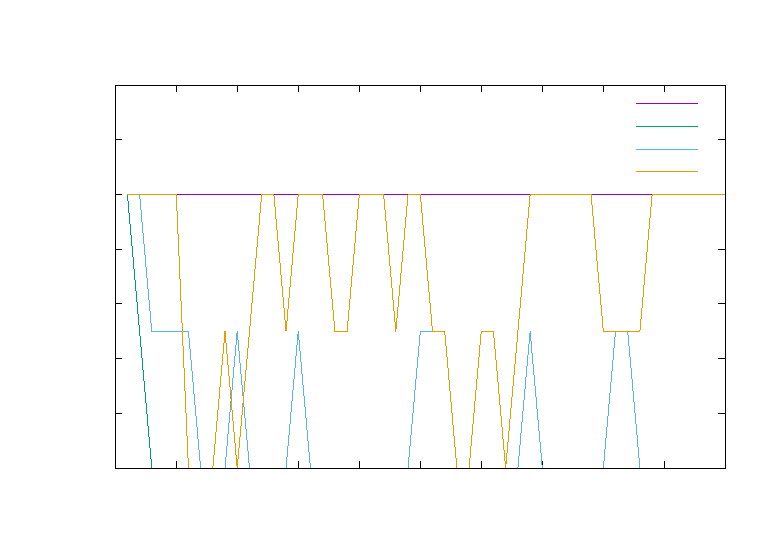
\includegraphics[width={360.00bp},height={252.00bp}]{neighbourhood}}%
    \gplfronttext
  \end{picture}%
\endgroup
 
\end {center}
\caption{Results from four 50 round tournaments with static agents
  with neighbourhood voting.  3-TFT refers to 3 tit-for-tat agents
  that start cooperating; they continue to cooperate.  2-TFT+D refers
  to two tit-for-tat agents with an agent that always defects; this
  quickly descends to no cooperation.  2-TFT-E+D refers to two
  tit-for-tat agents with 10\% exploration and an always defect agent;
  this system has some cooperations but mostly defects; note that it
  defects more than when there is pairwise voting.  2-TFT-E+C refers
  to two tit-for-tat agents with 10\% exploration and an agent that
  always cooperates; this cooperates about half the time, which is
  less than when there is pairwise voting.}
  \label{figStaticOneVote}
\end {figure}


The reason behind this is that the reward space for each agent tends
toward the positive when there is pairwise voting.  Each agent can
punish particular defectors and reward particular collaborators.  This
is why the agents can all get better results and ascend the
Collaborative Hill.  On the other hand, with neighbourhood voting,
each agent can only reward or punish in aggregate.  The reward structure is
that each agent does better by defecting, and any collaboration tends to
give worse immediate results.  This reward space and the agents' ability
to only weakly influence other agents draws the agents into the Tragic
Valley where agents do not cooperate.

Note that without exploration, the static policies move into an attractor
state.  When all three agents are TFT, if they all collaborate, they
will continue to do so;  not shown is the case when the initial choice
is random.  In the one of eight times when all three agents defect, the
system starts in the attractor state when they all defect, and continue
to defect.  In the case where there is mixed voting, the system will move
about until it gets to one of the two attractor states.

Figure \ref {figStaticAverage} compares the Tit-for-Tat agents with
exploration and voting mechanisms.  These are similar to the runs in
figures \ref {figStaticTwoVotes} and \ref {figStaticOneVote}, but
here the results reflect an average of 100 runs.  It indicates that
the pairswise voting strategy is more likely to collaborate in the
against always defect though this is eventually always collaboration
between the two Tit-for-Tat agents.

\begin{figure} [ht]
\begin{center}
\input {avg.tex} 
\end {center}
\caption{Results from the average of 100  50 round tournaments with four
  different sets of agents.  All the sets have two Tit-for-Tat (TFT) agents with
  10\%   exploration.  Two have a third agent that always defects, and
  two have one that always cooperates.  The other variable is
  voting (pairwise or neighbourhood).}
  \label{figStaticAverage}
\end {figure}


\section {Reinforcement Learning Agents}

The authors were suprised that they found no papers explicitly stating
that pairwise voting led to largely good performance.  However, this
may be due to pairwise voting being largely equivalent to
$(N-1)*(N-2)$ individual tournaments.  Thus, the original work on the
two person Prisoner's Dilemma holds.

Using standard Q-learning agents with only two steps of history,
agents become cooperative with two votes, and defect with one.

\begin{figure} [ht]
\begin{center}
\input {avgQ.tex} 
\end {center}
\caption{Results from the average of 100  500 round tournaments with two
  different sets of agents.  Both sets are two Q-Learning agents with
  one Tit-for-Tat agent with exploration.  They differ by pairwise
  vs. neighbourhood voting, and the average of the Q-Learning agents
  have a line, and the Tit-for-Tat agent has a line.  
  This clearly shows the pairwise agents remaining collaborative while
  the neighbourhood agents descend into the Tragic Valley.}
  \label{figQAverage}
\end {figure}

undone results from 5 7 19 and 25 agents

undone results of q-learning agents vs. always cooperate pairwise and
neighbour

\begin{table}
  \caption{System Parameters}
  \label{tableResults}
  
\begin {tabular}  {|c|c c|c c|}
\hline
Agent 1 and 2 Type & Average Cooperation & Agent 3 Type  & Average Cooperation \\
\hline
Pairwise &Q Learning& 85\%&TFT &80\%undone\\
\hline
\end {tabular}
\end{table}



\section{Escaping the Tragic Valley with Enhanced Reinforcement Learning}
\label{sec:enhanced_rl}

The preceding sections have established a critical dichotomy: the pairwise interaction model creates a "Collaborative Hill" where simple reciprocity can thrive, while the neighbourhood voting model leads to a "Tragic Valley" of mutual defection for both static agents (Section \ref{sec:tragicValley}) and basic reinforcement learners (Section \ref{sec:tragicValley}). The diffuse nature of rewards in the neighbourhood setting obscures the one-to-one accountability needed for simple learning algorithms to foster cooperation.

This raises a crucial question: is the Tragic Valley an inescapable feature of the N-IPD's neighbourhood structure, or can it be overcome by more sophisticated agents? To investigate this, we developed an "Enhanced Q-Learning" (EQL) agent, designed to better perceive and react to the dynamics of group behaviour.

\subsection{The Enhanced Q-Learning Agent}

The standard Q-learning agent, which bases its state on a simple discretization of the previous round's cooperation, struggles to identify meaningful patterns. Our Enhanced Q-Learning agent incorporates several key improvements inspired by advancements in MARL to create a more sophisticated learning mechanism:

\begin{itemize}
    \item \textbf{Richer State Representation:} Instead of just the previous round's cooperation level, the EQL agent's state can incorporate its own action history and the trend of group cooperation over multiple rounds. For example, a state might capture not only that cooperation is 'high', but also that it is 'stable' or 'increasing', and whether the agent itself has been cooperating or defecting. This allows the agent to learn the consequences of its actions on the group's trajectory.
    \item \textbf{Optimistic Initialisation:} The EQL agent's Q-table is initialised with optimistic values for unexplored state-action pairs \cite{SuttonBarto2018}. This encourages the agent to thoroughly explore its options, particularly cooperative actions, before committing to a potentially suboptimal defect-heavy strategy.
    \item \textbf{Adaptive Exploration:} The agent employs a decaying epsilon-greedy strategy. It explores more at the beginning of a tournament and gradually reduces its randomness to exploit the knowledge it has gained, allowing for convergence to a stable policy.
\end{itemize}

These enhancements transform the agent from a purely reactive learner into one that can perceive and respond to the emergent dynamics of the system.

\subsection{Comparative Results: Learning to Cooperate}

To test the EQL agent's capabilities, we ran a series of tournaments mirroring those in the previous sections. The results demonstrate a clear and significant ability to escape the Tragic Valley.

The most striking result is observed when placing a single EQL agent in a group with two Tit-for-Tat (TFT) agents. As established, a basic Q-learner in this scenario learns to exploit the initially cooperative TFTs, leading to a downward spiral of defection. The EQL agent, however, behaves entirely differently.

As shown in Figure \ref{fig:EQL_vs_TFT_neighbourhood}, the EQL agent learns to reciprocate the TFTs' cooperative nature. Its cooperation rate climbs and stabilises at a high level, resulting in a system of mutual cooperation. Crucially, its cumulative score rises in lockstep with the TFT agents, indicating it has discovered a high-payoff, cooperative equilibrium. This emergence of sustained cooperation, driven by a higher score, is precisely the intelligent behaviour we seek.

% --- Figure Placeholder ---
% create this figure by taking the top-right subplot from  "1 Enhanced QL Neighbourhood - Cooperation Rates" image
% and the top-right subplot from  "1 Enhanced QL Neighbourhood - Cumulative Scores" image and combining them
\begin{figure}[ht]
    \centering
    \includegraphics[width=\textwidth]{placeholder_EQL_vs_2TFT_neighbourhood.png}
    \caption{Performance of a single Enhanced Q-Learning (EQL) agent with two TFT agents in the neighbourhood setting (average of 500 runs). Left: The EQL agent's cooperation rate rises to match the TFT agents. Right: The EQL agent achieves a high cumulative score, comparable to the cooperative TFT agents, demonstrating it has learned a beneficial, cooperative policy.}
    \label{fig:EQL_vs_TFT_neighbourhood}
\end{figure}

The EQL agent also demonstrates rational behaviour in less cooperative environments. When paired with two "Always Defect" (AllD) agents, it quickly learns that cooperation is futile and its cooperation rate drops to the baseline exploration level (Figure \ref{fig:EQL_vs_AllD_AllC_neighbourhood}, left panel). This confirms the agent is not simply a blind cooperator; it is learning an appropriate, context-dependent strategy.

Interestingly, when placed with one AllD and one "Always Cooperate" (AllC) agent, the EQL agent learns to defect. (Figure \ref{fig:EQL_vs_AllD_AllC_neighbourhood}, right panel). It learns that cooperating does not influence the AllD agent and that defecting does not influence the AllC agent.

% --- Figure Placeholder ---
% create this figure by taking the top-left subplot ("1 EQL + 2 AllD") and the middle-right subplot ("1 EQL + 1 AllD + 1 AllC")
% from "1 Enhanced QL Neighbourhood - Cooperation Rates" image a
\begin{figure}[ht]
    \centering
    \includegraphics[width=\textwidth]{placeholder_EQL_vs_AllD_AllC_neighbourhood.png}
    \caption{Cooperation rate of an EQL agent in uncooperative neighbourhood settings. Left: Against two AllD agents, the EQL agent learns to defect.}
    \label{fig:EQL_vs_AllD_AllC_neighbourhood}
\end{figure}

These results show that the structural barrier of the Tragic Valley is not insurmountable. An agent equipped with a sufficiently rich state representation and a robust exploration mechanism can learn to identify and foster cooperative dynamics even in the absence of direct, pairwise reciprocity.


\section{Conclusion}
\label{sec:conclusion}

\fbox{undone something}


% --- Bibliography ---
\bibliographystyle{ieeetr} % Using a standard IEEE transaction style (numbered)
\bibliography{prisoners}   % Your .bib file is named prisoners.bib

% --- Appendix (Optional - if you want to keep your original Chapter 3/Results) ---
\begin{subappendices} % Using subappendices from appendix package
\label{app:original_results}


\end{subappendices}


\end{document}
